%-------------------------------------------------------------------------
%-------------------------------------------------------------------------
%-------------------------------------------------------------------------

\chapter[Appendix: Field Study]{Field Study Supplemental Material}
\label{app:overview}

%-------------------------------------------------------------------------
%-------------------------------------------------------------------------
%-------------------------------------------------------------------------

This appendix supports \autoref{ch:overview}. 
It contains the full scatterplot\index{visual encoding!scatterplot} from the {\sc warlogs} initial use case (Fall 2010, a detail was provided in \autoref{overview:fig:warlogs}), a screen shot of the {\it Overview v1}\index{Overview (document mining tool)} prototype (Fall 2011), our original project proposal (Spring 2012), our interview protocol (Spring 2012), preliminary field study results (Fall 2012), and a screen shot of {\it Overview v3}\index{Overview (document mining tool)} (Fall 2012).

\section{Initial Use Case}
\label{app:overview:initial-use-case}

%-------------------------------------------------------------------------
%-------------------------------------------------------------------------

The initial {\sc warlogs} use case, described in \autoref{overview:motivation}, resulted in the scatterplot\index{visual encoding!scatterplot} shown in \autoref{app:overview:fig:warlogs} (a detail is also shown in \autoref{overview:fig:warlogs}), which was produced by Jonathan Stray in Fall 2010~\cite{Stray2010}.

%-|-|-|-|-|-|-|-|-|-|-|-|-|-|-|-|-|-|-|-|-|-|-|-|-|-|-|-|-|-|-|-|-|-|-|-|-

\begin{figure}
	\centering
	\fbox{\includegraphics[width=0.975\textwidth]{figures/warlogs-full.png}}
	\caption
	[
	    \textsl{``A full-text visualization of the Iraq War Logs''}.
	]
	{
	    \textsl{``A full-text visualization of the Iraq War Logs''} (the {\sc warlogs} initial use case) by Jonathan Stray~\cite{Stray2010}.
	}
	\centering
	\label{app:overview:fig:warlogs}
\end{figure}

%-|-|-|-|-|-|-|-|-|-|-|-|-|-|-|-|-|-|-|-|-|-|-|-|-|-|-|-|-|-|-|-|-|-|-|-|-

%-------------------------------------------------------------------------
%-------------------------------------------------------------------------

\section{Overview v1}
\label{app:overview:v1}

%-------------------------------------------------------------------------
%-------------------------------------------------------------------------

\textsl{Overview v1}, a prototype desktop application completed in Fall 2011, is shown in \autoref{app:overview:fig:overview-v1}.

%-|-|-|-|-|-|-|-|-|-|-|-|-|-|-|-|-|-|-|-|-|-|-|-|-|-|-|-|-|-|-|-|-|-|-|-|-

\begin{figure}
	\centering
	\fbox{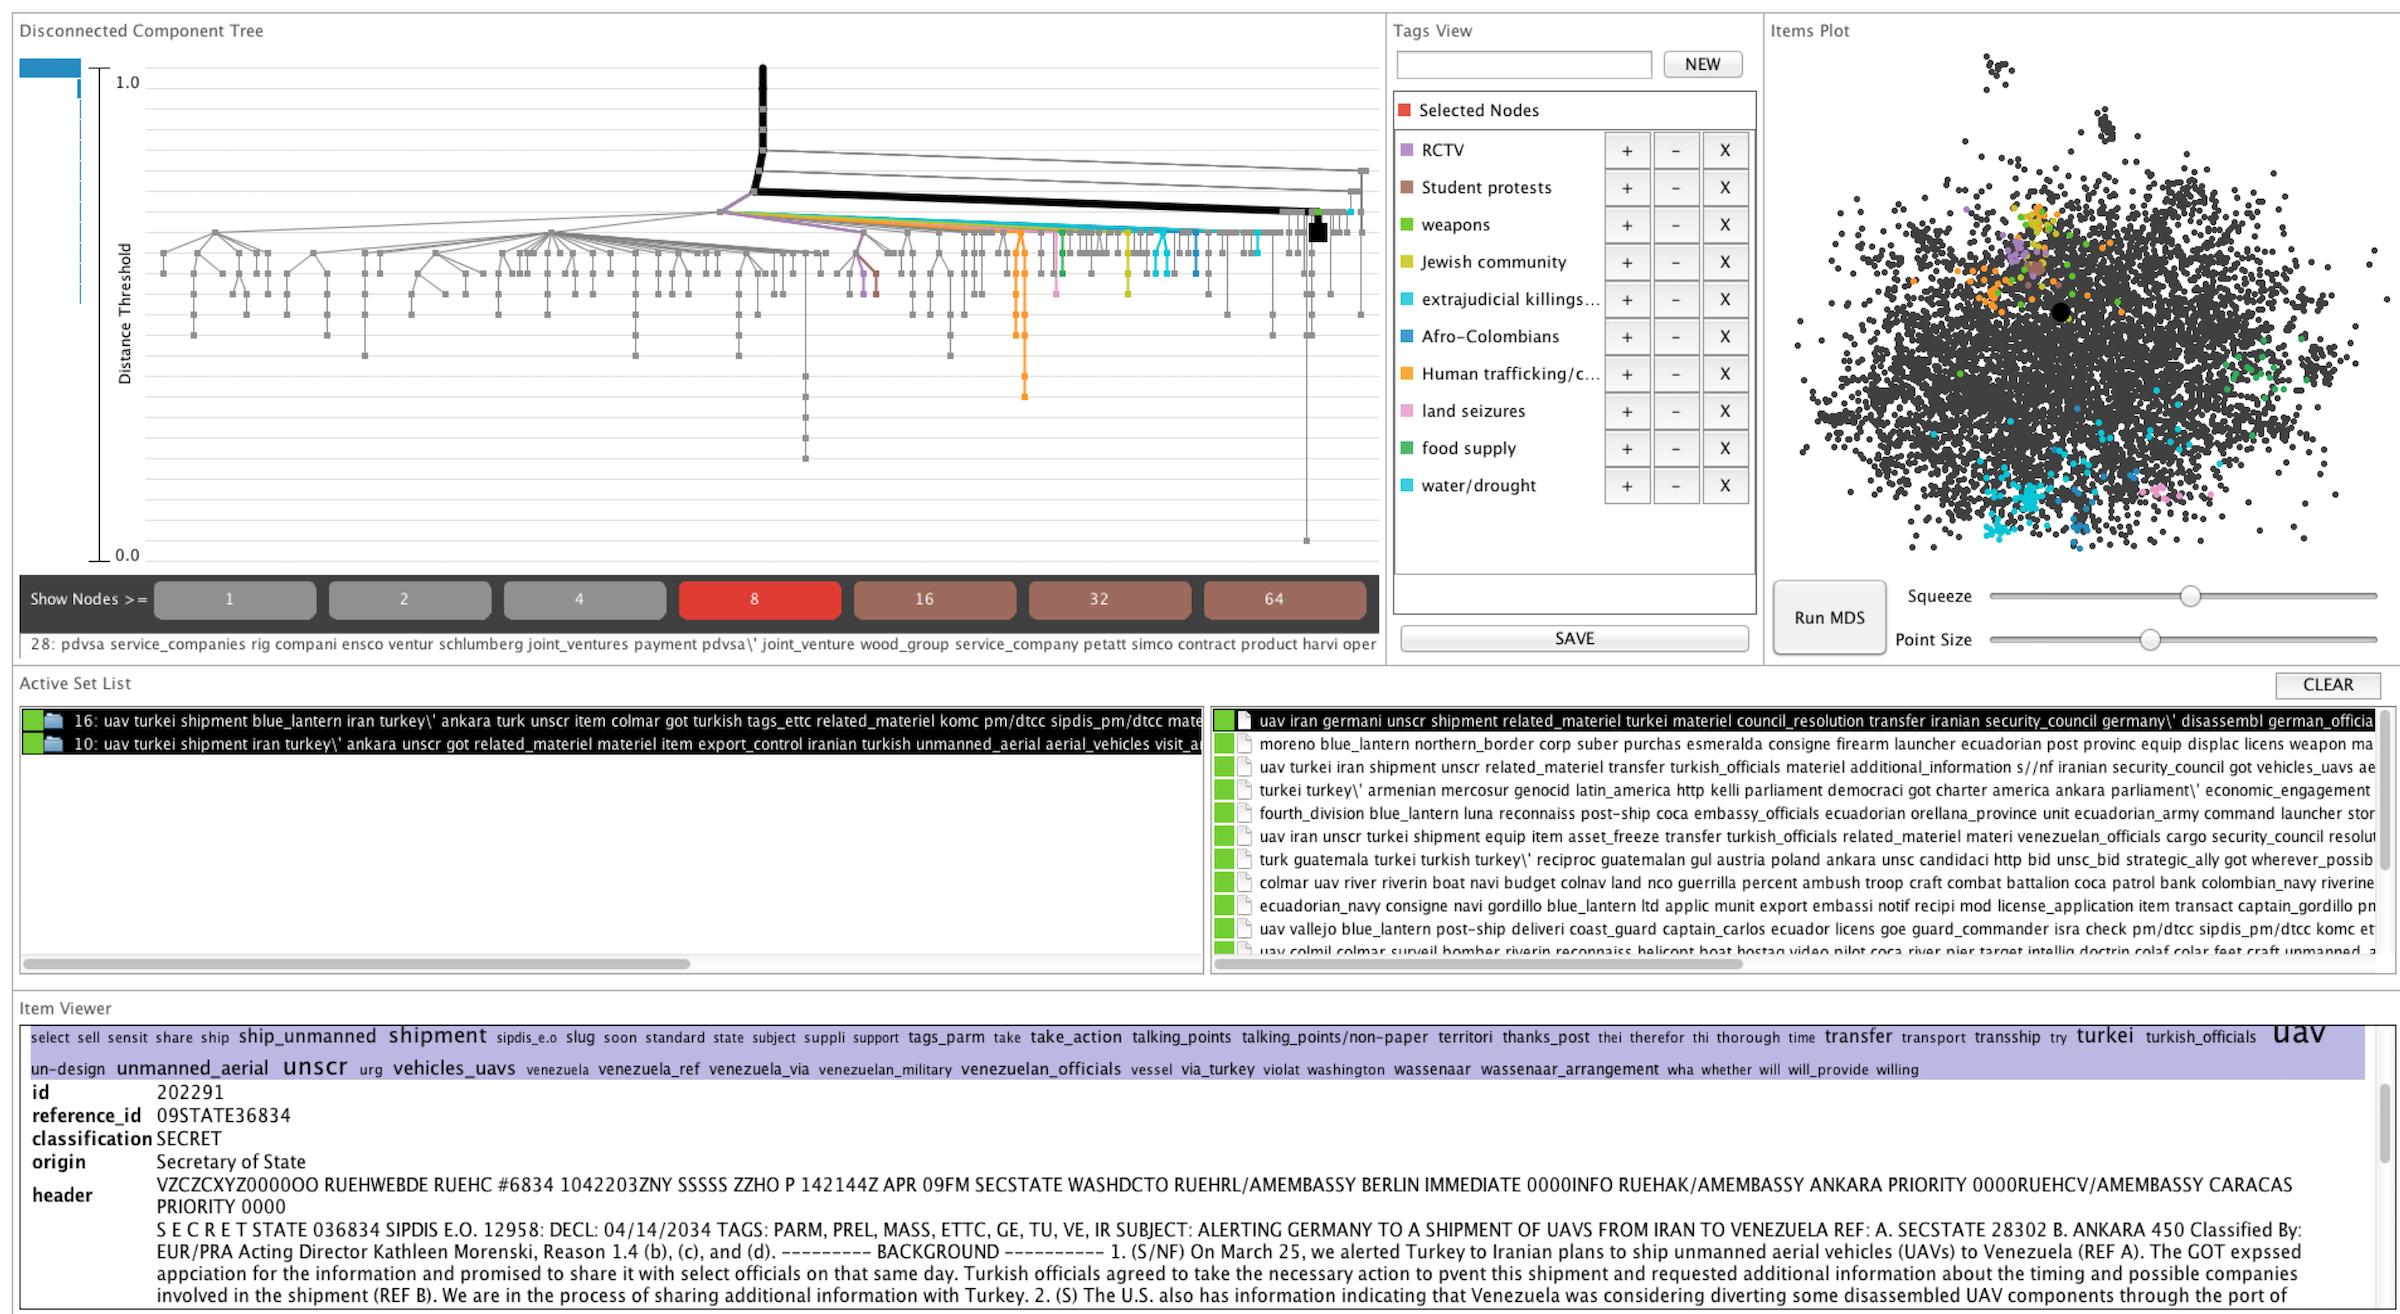
\includegraphics[width=0.975\textwidth]{figures/overview-v1.png}}
	\caption
	[
	    \textsl{Overview v1}, a prototype desktop application completed in Fall 2011.
	]
	{
    	\textsl{Overview v1}, a prototype desktop application completed in Fall 2011.
	}
	\centering
	\label{app:overview:fig:overview-v1}
\end{figure}

%-|-|-|-|-|-|-|-|-|-|-|-|-|-|-|-|-|-|-|-|-|-|-|-|-|-|-|-|-|-|-|-|-|-|-|-|-

%-------------------------------------------------------------------------
%-------------------------------------------------------------------------

\section{Field Study Proposal}
\label{app:overview:proposal}

%-------------------------------------------------------------------------
%-------------------------------------------------------------------------

\footnote{This research proposal for the {\it Overview}\index{Overview (document mining tool)} field study was written in April 2012.}In the fall of 2010, WikiLeaks released 391,832 text documents\index{document data} relating to the conduct of American armed forces and independent security contractors during the war in Iraq. 
Since that time, specialized investigative {\it data journalists}\index{journalism} have reported on what was contained in this vast deposit of documents\index{document data}, which included startling information regarding civilian casualties, friendly fire incidents, and observed breaches of protocol. 
My proposed research, in brief, asks how data journalists\index{journalism} {\it mine} such deposits, how they seek information to support or refute prior findings, or how they come to discover unanticipated yet newsworthy stories hiding in the data.

The motivation for this research proposal reflects the growing trend of large collections of emails, reports, and other documents\index{document data} being dumped, leaked, released, or declassified by corporations, government agencies, and other organizations, such as WikiLeaks. 
Fellow journalists\index{journalism} and the news-reading public deserve transparency when it comes to the methods of data journalists\index{journalism} who investigate these collections. 
Additionally, developers of data analysis applications require a better understanding of journalists\index{journalism} as potential adopters.

Aside from being a consumer of news media, I have no background in journalism\index{journalism}. 
Rather I represent the interests of application developers, and I am sensitive to theoretical concepts relating to the design of tools for supporting data analysis.
While this theoretical repertoire is useful for understanding low-level perceptual activity contributing to how individuals interact with data displays~\cite{Amar2005,Shneiderman1996}, or for understanding high-level domain-agnostic abstractions relating to information foraging and sensemaking~\cite{Amar2004,Pirolli2009}, I am faced with a gap in the middle. 
How can I characterize the data analysis process within the context of a domain such as journalism\index{journalism}? 
Moreover, how does this process play out with a specific type of data, in this case being collections of text documents\index{document data}? 
Thus I seek a middle-level theory to explain this process.

%-------------------------------------------------------------------------
\subsection{Research Questions}
\label{app:overview:proposal-questions}
%-------------------------------------------------------------------------

My predominant research question asks: What is document mining\index{document mining}? 
That is, how do journalists\index{journalism} conduct data analysis when faced with more documents\index{document data} than they could possibly read in a year, let alone in time to meet a deadline?

Several additional questions follow from this: namely, what constraints do these journalists\index{journalism} face in the process of their work? 
What tools do they use and how do they use them? 
Do they collaborate with other people, and if so, how do they collaborate?

Finally, this work will determine how document mining\index{document mining} compares to other analytical processes in data journalism\index{journalism}, when the data is comprised of numbers rather than text documents\index{document data}, which could include large financial databases or historical measurements. 
I will also make comparisons between document mining\index{document mining} and other processes of investigative journalism\index{journalism}, as well as with processes of data analysis characterized in other domains, such as business intelligence and law enforcement.

%-------------------------------------------------------------------------
\subsection{Research Context}
\label{app:overview:proposal-context}
%-------------------------------------------------------------------------

Journalists\index{journalism} engaging in document mining\index{document mining} are found in newsrooms around the world. 
Unfortunately, like many busy professionals, they are often working under tight deadlines, and have little time to participate in academic research. 
However, I am lucky enough to know someone ``on the inside''.

Jonathan Stray is a computer-scientist-turned-journalist\index{journalism} now employed by the Associated Press, based out of New York City. 
Working in collaboration with my research group, he has developed {\it Overview}\index{Overview (document mining tool)}, a robust data visualization application for document mining\index{document mining}, recently made available as a free download\footnote{Recall that {\it Overview v2} was a desktop application (\url{https://github.com/overview/overview-prototype}), which was later replaced by the {\it v3-v4} web application.}. 
He is currently\footnote{As of Spring 2012.} pitching {\it Overview}\index{Overview (document mining tool)} to journalists\index{journalism} via conferences, workshops, and social media. 
Buzz surrounding {\it Overview}\index{Overview (document mining tool)} is starting to grow in the data journalism\index{journalism} community.

Stray is our gatekeeper to research participants, as his potentially useful application provides an incentive for journalists\index{journalism} participate in our research. 
As a result, we have an opportunity to satisfy two research goals: (1) assess whether {\it Overview}\index{Overview (document mining tool)} is usable and useful, as well as how it fits within existing document mining\index{document mining} workflows\index{workflows}; and (2) characterize the process and context of document mining\index{document mining}, with and without this new application. 
While this proposal focuses on the latter goal, data collection corresponding to both goals will occur simultaneously. 
Furthermore, it is my intent that in working toward the second goal, my findings will contribute to the future development of {\it Overview}\index{Overview (document mining tool)} and other applications like it.

Due to the distributed nature of this research, logistical constraints will keep me from visiting individual journalists\index{journalism} in newsrooms. 
Thus my data collection will occur at a distance, over the phone and online.

%-------------------------------------------------------------------------
\subsection{Methodology}
\label{app:overview:proposal-methodology}
%-------------------------------------------------------------------------

A need to characterize the process of document mining\index{document mining} among journalists\index{journalism} necessitates a grounded theory approach~\cite{Charmaz2006}\index{grounded theory}. 
This approach is in turn informed by an interpretivist, symbolic interactionist theoretical perspective and a constructionist epistemology~\cite{Crotty1998}. 
That is, I intend to focus on the language used by journalists\index{journalism} to describe this process, and construct a shared interpretation of this process based on interactions with research participants and the data they generate.

The constant comparative method of grounded theory\index{grounded theory} will allow me to flexibly make comparisons between the process of document mining\index{document mining} with other journalistic processes, as well as processes relating to data analysis in other domains. 
Comparisons will also be made between journalists\index{journalism}, between newsrooms, and over periods of time. 
For instance, I will be comparing the process of document mining\index{document mining} both before and after the introduction of {\it Overview}\index{Overview (document mining tool)}, the new visualization tool.

A further justification for the use of a grounded theory\index{grounded theory} methodology is that my initial research questions are not theoretically deduced hypotheses. 
Rather, my questions are informed by sensitizing concepts and assumptions held within my domain. 
It is these sensitizing concepts that allowed me to frame the data collection methods, particularly a preliminary set of interview questions.

These sensitizing concepts include the notion that data analysis, document mining\index{document mining} being an instance of which, occurs in stages. 
Data analysis may involve stages of hypothesis generation, each necessitating an exploration of the data without a particular set of questions in mind, save perhaps ``What's going on here?'' 
Other times there may be stages of hypothesis validation, where the goal is to support or refute prior evidence. 
These stages necessitate a directed search within a subset of the data, or a comparison between individual items or documents\index{document data}. 
Individuals may or may not engage in both types of stages during the course of a single investigation.

The products of data analysis are also among my sensitizing concepts. 
These products include {\it ``Eureka!''} moments of insight\index{insight}, serendipitous discoveries, and both optimal and suboptimal solutions to closed- and open-ended problems. 
Admittedly, these products of analysis are ill-defined constructs, and it will be necessary to attain our research participants' interpretations of their meaning, as well as their native terminology.

Finally, these sensitizing concepts include the disentanglement of an individual's expertise. 
By this I mean that an analyst may have expertise within a domain, expertise using specific analytical tools or techniques, and/or expertise regarding the data, its semantics and its provenance.

In my field of research, there exist several precedents for the use of grounded theory\index{grounded theory}, or at least the use of methods inspired by a grounded theory\index{grounded theory} methodology. 
The methodology has informed prior work which has characterized the data analysis processes of professionals in other domains, including architecture~\cite{Tory2008} and national security and intelligence~\cite{Kang2011}. 
There also exists a grounded evaluation\index{evaluation} method for determining the effectiveness of visualization software when deployed in target contexts of use~\cite{Isenberg2008}. 
Both uses of grounded theory\index{grounded theory} methods serve as inspiration for my proposed research.

\bstart{Data collection methods and sources}
My primary data collection method will be intensive, open-ended interviews with journalists\index{journalism}. 
These interviews will be teleconferences or group Skype chats. 
Both Stray (in New York City), and myself (at UBC) will have questions to ask interviewees, with his questions pertaining to the usability and utility of {\it Overview}\index{Overview (document mining tool)}. 
Audio from these interviews will be recorded for later transcription.

Following the methodology of grounded theory\index{grounded theory}, I will not specify the number of interviews that I plan to conduct a priori. 
The final number of interviews will depend on how much theoretical sampling is required before achieving data saturation, the point where no new categories emerge; I will return to this point below when I discuss data analysis methods. 
The number of interviews will also depend on how many journalists\index{journalism} download and use {\it Overview}\index{Overview (document mining tool)}, and among those, how many express a willingness to participate in interviews. 
Ideally, I would like to perform multiple interviews with each journalist\index{journalism} in order to make comparisons over time, as their processes vary or change over time, before, during, and after using the new tool. 
However, this is an unrealistic plan. 
As mentioned in \autoref{app:overview:proposal-context}, these journalists\index{journalism} will often be conducting their investigation and writing their story under a tight deadline, and will likely only have time to commit to an intensive interview after the story is written. 
As a result, I will rely on secondary data collection methods, such as follow-up email exchanges, to fill in some of the gaps. 
These methods are discussed in greater detail below.

Regarding the content of these interviews, I plan to keep the number of initial questions small. 
I have prepared a list of interview foci with a small set of representative questions for each, composed according to guidelines for open-ended interviews~\cite{Fontana1994} and for interviews conducted in the context of a grounded theory study~\cite{Charmaz2006}\index{grounded theory}. 
These foci correspond with the research questions mentioned above in \autoref{app:overview:proposal-questions}. 
In particular, I will attempt to ground the interview in the interviewee's example of document mining\index{document mining}, one drawn from their prior experience. 
This will invite comparisons with other journalistic processes\index{journalism}, as well as comparisons between their processes before and after their initial use of {\it Overview}\index{Overview (document mining tool)}.

Many questions are redundant and cross-referential, a deliberate choice, as I have no intention to ask all or even most of them in a single interview. 
An answer to one open-ended question is expected to answer many of the others; these foci and questions are more so a checklist than a script. 
I also expect this list of foci and questions to change as I conduct interviews, as a result of theoretical sampling and the possibility that early interviews will illuminate unanticipated themes and concepts.

I plan to complement the interviews by eliciting texts and other information from journalists\index{journalism} that I interview. 
Follow-up questions will be asked via email. 
I will also request copies of the notes journalists\index{journalism} take during the course of their investigation. 
I expect that in many cases, journalists\index{journalism} will be taking notes regardless of whether or not I ask to see them. 
I will also request information regarding the data, such as how many documents\index{document data} are contained in the document collection\index{document data} being investigated, how they tend to vary from one another, how many were read or skimmed during the course of their investigation, how many were discarded or ignored, as well as why individual documents\index{document data} were read, skimmed, ignored, or discarded. 
In cases where these documents\index{document data} are publicly available, I will examine the documents\index{document data} as well. 
Screenshots or pictures of annotated documents\index{document data}, journalist\index{journalism} notes, and other analytical artifacts, such as spreadsheets or charts, will also be requested.

Realizing the value of found data~\cite{Silverman2007}, I will also collect several extant texts. 
In particular, I will collect the stories journalists\index{journalism} write as a result of their investigations. 
I will examine the extent to which the document\index{document data} mining process is transparent in their articles, allowing for a comparison with their notes and the remarks they make during interviews. 
Finally, in cases where these stories are published online, I will also collect the reader perspective, via comments and discussion boards.

\bstart{Data analysis methods}
Data collection and analysis for this project will occur concurrently. 
Interviews and artifacts collected from journalists\index{journalism} will be subject to multiple iterations of coding\index{coding (qualitative data analysis)}, each calling upon the constant comparative method, the basis of grounded theory~\cite{Charmaz2006}\index{grounded theory}. 
First, open coding\index{coding (qualitative data analysis)} will label the data, at the line or paragraph level, using words or short phrases used in the data. 
Next, tentative categories of codes will be generated, each with an explanatory rationale based on comparisons between code instances, recorded in memos. 
This will inform subsequent data collection and focused coding\index{coding (qualitative data analysis)}. 
The process of axial coding\index{coding (qualitative data analysis)} follows, a recoding of the data using the categories constructed. 
At this point, the process of theoretical sampling will direct me to specific data collection, using different interview foci or artifact collection criteria. 
As categories become refined and theoretical concepts emerge through the process of selective coding\index{coding (qualitative data analysis)} and memoing, I will begin to seek theoretical saturation, the point where no unexamined concepts are apparent. 
At this time, I will begin to construct a mid-level theory of document mining\index{document mining} based on the relationships between concepts. 
This stage will also involve comparisons between my theory and other theories of data analysis, as it occurs in other domains and as it is described at higher levels of abstraction~\cite{Amar2004,Pirolli2009}.

Triangulation between researchers is highly effective during interpretive analysis~\cite{Mathison1988}. 
I will share my findings with Stray. 
While he and I have different foci and research goals, we will both be engaged in participant interviews, and thus can compare notes. 
Additionally, his own journalistic\index{journalism} expertise can also be called upon throughout the stages of my analysis.

I will also triangulate in terms of methods, in that I will take an alternative approach to thematic coding~\cite{Ryan2003}\index{coding (qualitative data analysis)}. 
This will involve an examination of word frequency, word co-occurrence, key words as used in context, linguistic connectors, and metaphors used. 
Extant texts and artifacts collected will also be analyzed in terms of their descriptive properties, as well as their intellectual and cultural values~\cite{Prown1982}. 
I will then compare the codes produced by these alternative methods to the codes and categories generated via the grounded theory\index{grounded theory} methods.

%-------------------------------------------------------------------------
\subsection{Outcomes and Follow-on Work}
\label{app:overview:proposal-outcomes}
%-------------------------------------------------------------------------

I anticipate two audiences to which I will report my findings. 
The first are readers of peer-reviewed academic publications and/or conference proceedings in the fields of \ac{HCI}\index{human-computer interaction (HCI)}, visualization, and visual analytics\index{visual analytics}. 
The second audience for my findings are journalists\index{journalism} and the news-reading public, so I plan to report my findings online, either via my own website or in collaboration with the Associated Press.
I hope to apply my findings in the future development of {\it Overview}\index{Overview (document mining tool)} and other
applications like it. 
Finally, I anticipate that an examination of what makes {\it Overview}\index{Overview (document mining tool)}
ultimately successful or unsuccessful will call for a critical inquiry of existing values and standards in journalism\index{journalism}, as well as existing theories of data analysis.

%-------------------------------------------------------------------------
%-------------------------------------------------------------------------

\section{Interview Protocol}
\label{app:overview:interview-protocol}

%-------------------------------------------------------------------------
%-------------------------------------------------------------------------

The interview foci and associated questions below can be lumped into two broad categories: understanding the data journalist\index{journalism} and understanding their use of {\it Overview}\index{Overview (document mining tool)}\footnote{This exhaustive list of questions, drafted in Spring 2012, proved to be impractical as a script in actual interviews; despite this, answers to many of these questions arose naturally in conversation.}. 
In semi-structured interviews, some questions come about naturally as follow-on questions, so this list is by no means a linear interview script; these questions are intended to be asked during / after a screen-sharing walkthrough.

\bstart{Utility and efficacy}

\begin{itemize}
    \item What (have / are) you (used / using) {\it Overview}\index{Overview (document mining tool)} to do?
    \item Can {\it Overview}\index{Overview (document mining tool)} ingest some or all of your data? How long did this take? How much time did you spend cleaning/formatting the data specifically for {\it Overview}\index{Overview (document mining tool)}?
    \item How did you explore your data using {\it Overview}\index{Overview (document mining tool)}? How long did this take?
    \item How did you search your data using {\it Overview}\index{Overview (document mining tool)}? How long did this take?
    \item Did you have hunches about a story a priori? Were you able to verify these hunches?
    \item Did you develop new hunches about your story while using {\it Overview}\index{Overview (document mining tool)}?
    \item How did you choose which documents\index{document data} to read? Depth vs. breadth? How long did you spend employing these strategies? How many individual documents\index{document data} did you skim / read?
    \item How did you go about tagging your data in {\it Overview}\index{Overview (document mining tool)}? How long did this take? How many tags did you generate? How many did you delete? How many did you consolidate / split? How many of these tags were structural vs. semantic?
    \item What level(s) of tree\index{visual encoding!tree} pruning\footnote{In {\it Overview v1-v2}, recall that tree pruning was controlled globally for the entire tree\index{visual encoding!tree}, and not selectively for each interior node; see \autoref{overview:rationale}.} were used? 
    \item Context of use: where were you while using {\it Overview}\index{Overview (document mining tool)}? What other applications did you have running? Were you taking handwritten or digital notes? Were you using {\it Overview}\index{Overview (document mining tool)} alone or in collaboration with others?
    \item How long did you use {\it Overview}\index{Overview (document mining tool)} for? How long was spent reading documents\index{document data} vs. organizing, browsing / sorting / tagging?
    \item Did this match your time frame expectation prior to using {\it Overview}\index{Overview (document mining tool)}, given the size of the dataset?
    \item How much time was spent reading a single document? Did this vary?
    \item What proportion of documents\index{document data} did you read/skim? Are you confident in this proportion? Why or why not?
    \item What proportion of documents\index{document data} did you tag? Are you confident in this proportion? Why or why not?
    \item Not enough tags vs. too many tags?
    \item How did you deal with (unique / weird / important / unimportant / relevant / irrelevant) documents\index{document data}? (these may be overlapping categories).
    \item How did you dismiss the unimportant? The irrelevant and unimportant?
    \item Did you ever flag documents\index{document data} for later follow-up? Did this eventually happen?
    \item Did you ever re-read documents\index{document data}? Was this intentional?
    \item How, if at all, did you use the sampling functionality\footnote{This feature from {\it Overview v2} randomly chose a document from selected node, highlighted it in each view, and displayed the document in the {\it Document Viewer}.} to read documents\index{document data}? 
\end{itemize}

\bstart{Usability}

\begin{itemize}
    \item On installing {\it Overview}\index{Overview (document mining tool)}.
    \item On pre-processing data / ingesting data.
    \item Your first use of {\it Overview}\index{Overview (document mining tool)}: Orienting yourself within the \ac{UI}.
    \item Usability issues with respect to: Linked displays (selecting items); the tree\index{visual encoding!tree} display; the \ac{MDS}\index{dimensionality reduction (DR)!multi-dimensional scaling (MDS)} display\footnote{The scatterplot featured in {\it Overview v1-v2}.}; \ac{UI} for sampling; \ac{UI} for tagging; \ac{UI} for reading / opening in the browser\footnote{As {\it Overview v2} was a desktop application, it included a feature to open a document in a web browser as opposed to displaying its raw text content, provided that a document url was included in input data.}.
    \item What UI features did you like? Which didn't you like?
\end{itemize}

\bstart{Learnability}

\begin{itemize}
    \item Learning materials: Self-exploration vs. relying on Jonathan Stray's blog posts and instructions\footnote{These instructions have evolved since 2012; up-to-date instructional blog posts can be found here: \url{https://blog.overviewdocs.com/help/}.}, other sources? How much time spent on each?
    \item Developing a conceptual understanding of item layouts in the \ac{MDS}\index{dimensionality reduction (DR)!multi-dimensional scaling (MDS)} display and the tree\index{visual encoding!tree} display. 
\end{itemize}

\bstart{Adoption}

\begin{itemize}
    \item Has {\it Overview}\index{Overview (document mining tool)} become part of your workflow\index{workflows}?
    \item (If not), do you foreseeing it becoming part of your workflow\index{workflows}? Will it replace / add to / complement your workflow\index{workflows}?
    \item How often is there a document set where {\it Overview}\index{Overview (document mining tool)} could be used?
    \item Would you recommend use of {\it Overview}\index{Overview (document mining tool)} for colleagues? Do you expect them to you use it in their workflows\index{workflows}?
    \item Has {\it Overview}\index{Overview (document mining tool)} improved your process? Do you see {\it Overview}\index{Overview (document mining tool)} as having the potential to improve your process?
    \item Problems left unaddressed: What can't {\it Overview}\index{Overview (document mining tool)} do for you? What problem remains unaddressed?
    \item Previously untouched data: Were you able to ingest/analyze data that you couldn't approach with other tools?
    \item Previously unapproachable tasks\index{task}: Were you able to perform tasks\index{task} with {\it Overview}\index{Overview (document mining tool)} that you couldn't do (or couldn't do efficiently) with other tools?
    \item Discoveries with {\it Overview}\index{Overview (document mining tool)}: Have you made discoveries (in your data) using {\it Overview}\index{Overview (document mining tool)} that you wouldn't have been able to make with other tools?
\end{itemize}

\bstart{Personal background}

\begin{itemize}
    \item Who: What is your background and expertise?
    \item What brought you to working in this type of journalism\index{journalism}?
    \item Relevant demographic information: Age, number of years working in journalism\index{journalism}, number of years working in data journalism\index{journalism}, educational background.
    \item How did you become versed in {\it data journalism\index{journalism}}? Self-educated vs. formally educated, trained, or mentored, mixed (discerning between what was formally taught and what was independently learned). 
    \item Technical skill set: Spreadsheets and table manipulation, data cleansing, internal and external validation; programming / scripting experience.
    \item Skill set with respect to document mining\index{document mining} and unstructured data vs. skill set with respect to structured data.
\end{itemize}

\bstart{Context}

\begin{itemize}
    \item Tell me about your current day-to-day work.
    \item Career context: Agency / bureau affiliation, past and present.
    \item Spatial context: Where does the work happen? (Office setting, working remotely, other).
    \item Task\index{task} context: What else is going on? Multi-tasking vs. single-task\index{task} focus?
    \item Temporal context: Project time frame, deadlines: hours, days, weeks, months, vs. ongoing investigation.
\end{itemize}

\bstart{Collaboration}

\begin{itemize}
    \item To extent is the work collaborative? With respect to data acquisition, data pre-processing, analysis, writing, reliance on technical expertise of colleagues.
\end{itemize}

\bstart{Workflows and processes}

\begin{itemize}
    \item I'd like to hear about a recent story of yours, one from before using {\it Overview}\index{Overview (document mining tool)}, involving large collections of documents\index{document data}, representative of this type of work.
    \item (If there is no precedent) can I hear about a story involving large amounts of data analysis? Is this example representative or unique? (please provide links to articles, or send manuscripts).
\end{itemize}

\bstart{Methodology}

\begin{itemize}
    \item What was your data collection and analysis methodology prior to {\it Overview}\index{Overview (document mining tool)}? Personal vs. adopted / taught? Strictly followed protocol vs. ad hoc variations, subject to constraints of data, deadlines?
\end{itemize}

\bstart{Tool use}

\begin{itemize}
    \item What tools/services do you use for data collection (\eg DocumentCloud\footnote{\url{http://documentcloud.org/}})?
    \item How long does it take to collect data, using these tools/services?
    \item What tools do you use for pre-processing? Scraping / separating PDFs or semi-structured text? Cleansing? Internal and external validation (\eg Google Refine\footnote{Now OpenRefine: \url{http://openrefine.org/}}, Google Fusion\footnote{\url{https://goo.gl/DPj2pG}} tables, spreadsheet manipulation)?
    \item How long do these processes take, using these tools?
    \item What analysis tools do you use? (\eg tools for keyword search, data exploration / orientation, visualization?). 
\end{itemize}

For each tool:

\begin{itemize}
    \item What did you use the tool to do?
    \item Were you able to ingest some or all of your data? How long did this take? How much time did you spend cleaning / formatting the data specifically for this tool?
    \item How did you explore your data using this tool? How long did this take?
    \item How did you search your data using this tool? How long did this take?
    \item Did you have hunches about a story a priori? Were you able to verify these hunches? 
    \item Did you develop new hunches about your story while using this tool?
    \item How did you choose which documents\index{document data} to read? Depth vs. breadth? How long did you spend employing these strategies? How many individual documents\index{document data} did you skim / read?
    \item Context of use: Where were you while using this tool? What other applications did you have running? Were you taking handwritten or digital notes? Were you using this tool alone or in collaboration with others?
    \item How long did you use this tool for?
    \item Usability issues? Installing this tool? Pre-processing data / ingesting data? What was your first use of this tool like? How did you orient yourself within the \ac{UI}? What \ac{UI} features did you like? Which didn't you like?
\end{itemize}

\bstart{Data}

\begin{itemize}
    \item When collecting the data, what state was it in?
    \item Individual documents? Single document?
    \item When analyzing the data, what state is it in?
    \item Unstructured text vs. mixed / semi-structured vs. structured? For the latter two, categorical variables, numerical variables, a mixture?
    \item Are individual points (documents) tagged or untagged? For structured data, do categorical variables exist to tag each point?
    \item How do you find correlations between structured and unstructured information?
\end{itemize}

\bstart{Data provenance}

\begin{itemize}
    \item Where did the data come from? Who manufactured it? Who collected it or consolidated it?
    \item Who did the cleansing / pre-processing of the data (if not yourself)? 
    \item (If tags are used), where did the tags come from?
\end{itemize}

\bstart{Orientation}

\begin{itemize}
    \item Regarding orientation, by which I mean getting an initial overview of a dataset of unstructured text documents\index{document data}, how do you orient yourself within a dataset? Does orientation matter?
    \item How do you get a sense of the high-level structure of a dataset? The size of a dataset?
    \item To what extent do you rely on metadata? Tags? Word counts? Word co-occurrences? Word clouds? Word frequency? Mapping (when points have a geographical component)?
\end{itemize}

\bstart{Exploration vs. targeted search}

\begin{itemize}
    \item Relative time spent exploring vs. targeted search?
    \item How much of your work is hypothesis generation / exploration and how much is verification / fact checking?
    \item What other sources were used to complete the work? Other texts / data, vs. communications / interviews with people.
    \item When were other sources used? For hypothesis generation? For fact-checking/verification/corroboration? What was the pipeline/workflow\index{workflows} for using other sources?
\end{itemize}

\bstart{Results}

\begin{itemize}
    \item What constitutes a strong piece of data journalism\index{journalism} involving document mining\index{document mining}?
    \item Reader perspective: How should readers react to document mining\index{document mining} in journalism\index{journalism}? What do the reader comment boards say?
    \item Peer perspective: How should document mining\index{document mining} and by extension data journalism\index{journalism}, its goals and processes, be reviewed and critiqued be peers? How has your data journalism\index{journalism} been reviewed / critiqued?
\end{itemize}

%-------------------------------------------------------------------------
%-------------------------------------------------------------------------

\section{Preliminary Field Study Results}
\label{app:overview:preliminary-results}

%-------------------------------------------------------------------------
%-------------------------------------------------------------------------

\footnote{This report, written in September 2012, describes preliminary findings from the {\sc iraq-sec} and {\sc tulsa} case studies.}A post-deployment evaluation\index{evaluation} of a visualization tool can be difficult to conduct, particularly when evaluation\index{evaluation} criteria is contingent on determining how domain-specific professionals use the tool in the context of their ongoing work. 
Remote collaborators and journalists add to the logistical complexity of these evaluation\index{evaluation} studies. 
Such is the case with {\it Overview}\index{Overview (document mining tool)}, a visualization tool for exploring large document corpuses\index{document data}, built by our collaborator at the Associated Press. 
In this report I reflect upon the process and findings of an ongoing post-deployment, mixed-method evaluation\index{evaluation} of {\it Overview}\index{Overview (document mining tool)}, which includes an in-depth case study\index{case study} of a journalist\index{journalism} who used {\it Overview}\index{Overview (document mining tool)} to investigate a large email corpus. 
I also reflect upon how this work factors into my long-term research goals relating to exploratory data analysis and evaluation\index{evaluation} in visualization.  

%-------------------------------------------------------------------------
\subsection{Introduction}
\label{app:overview:prelim-intro}
%-------------------------------------------------------------------------

An evaluative\index{evaluation} study or experiment helps us to gauge the efficacy of a visualization tool or technique.
The prominence of evaluation\index{evaluation} in information visualization research has grown in recent years. 
A recent survey~\cite{Lam2012} of over eight hundred articles published between 1995 and 2010 at four major visualization venues reported an increasing trend of papers containing an evaluation\index{evaluation} component. 
The vast majority of these evaluation\index{evaluation} studies focus on usability or graphical perception issues. 
However, there has yet to be a similar increase in the number of papers reporting an evaluation\index{evaluation} of visualization users' context-dependent processes.
Evaluating\index{evaluation} users' processes with and without visualization can be highly informative at both formative and summative stages of visualization tool development~\cite{Andrews2008,Ellis2006}. 
Yet these evaluation\index{evaluation} studies tend to be time-consuming and costly, posing many logistical challenges, particularly when collaborators and users outside of academia are involved~\cite{Sedlmair2011}. 
As a result, post-deployment or summative evaluation\index{evaluation} studies are rarely published, and often report negative results~\cite{Gonzalez2003a,Munzner2011a}.

Novel evaluation\index{evaluation} methodologies and methods are emerging to overcome the challenges associated with studying user processes. 
In 2006, a workshop~\cite{Bertini2008} was established to discuss visualization evaluation\index{evaluation} {\it beyond time and error}, the historical metrics of usability and graphical perception studies. 
These metrics cannot be used to reliably answer our process-centric evaluative\index{evaluation} questions, nor can we rely upon controlled laboratory settings, prescribed experimental tasks\index{task}, or research participants who are unrepresentative of an intended user population~\cite{Carpendale2008,Plaisant2004,Sutcliffe2000}. 
Instead, the novel evaluation\index{evaluation} research community has established alternative metrics, conducting studies in externally valid research settings with representative users.
This community has proposed methods for measuring gains in insight~\cite{Saraiya2005b,Saraiya2006}\index{evaluation!insight-based evaluation}\index{insight}, for comparing problem-solving strategies~\cite{Mayr2010}, and for assessing how visualization tools can facilitate multiple forms of learning~\cite{Chang2010}. 
They have demonstrated that evaluation\index{evaluation} methodologies that incorporate qualitative data collection and analysis methods adopted from the social sciences can be rigorous, inductive, and replicable~\cite{Isenberg2008,Kang2011,Tory2008}.
Finally, they have shown that valid and reliable evaluation\index{evaluation} research often requires time, patience, and longitudinal coordination with collaborators and users~\cite{Lloyd2011,Saraiya2006,Shneiderman2006}.

The work I discuss in this report, a preliminary evaluation\index{evaluation} of a visual document mining\index{document mining} tool, has been motivated by my interest in the proliferation of emerging evaluation\index{evaluation} methodologies and methods. 
I am also motivated by my interest in how people perform exploratory data analysis with visualization tools or techniques: I want to know how visualization techniques or tools is used to solve ill-defined problems, to discover and understand, rather than to lookup and verify~\cite{Marchionini2006}. 
One way I like to describe this process is how someone who visualizes data may not know a priori what they are looking for in a dataset, but they'll know it when they see it. 
I want to be able to reliably evaluate\index{evaluation} how a visualization tool supports this process of serendipitous discovery. 

A fair question at this point is one of granularity: how do you define the process of exploration and discovery? 
There exists a body of work that characterizes these processes from an abstract, top-down perspective of human cognition~\cite{Amar2004,Pirolli2009,Springmeyer1992,Valiati2006}, while others have observed and characterized these processes from a bottom-up perspective, at the level of interface events~\cite{Amar2005,Shneiderman1996,Valiati2006,Winckler2004}. 
Task\index{task} taxonomies constructed either on abstract models of human cognition or on interface-level events can be helpful, but all too often they can be stifling if they are meant to be used as evaluation\index{evaluation} criteria~\cite{Beaudouin-Lafon2004}. 
This is particularly true when one is required to compare how people interact with different visualization tools across domains. 
A valid and comparative evaluation\index{evaluation} methodology requires a robust mid-level task\index{task} characterization of exploratory data analysis, one that spans domains and tool interfaces. 

My long-term goal is to contribute to the construction of such a task\index{task} characterization. 
To do this, I will study exploratory data analysis as it occurs across multiple domains, the tools individuals use, and the processes they undertake, while assessing how these tools and processes succeed or fail. 
I will employ a repertoire of established and emerging data collection and analysis methods, while reflecting upon the efficacy of my methodological choices.
This endeavour began in March of this year, studying journalists'\index{journalism} use of a visualization tool for exploring large document corpuses\index{document data}. 

%-------------------------------------------------------------------------
\subsection{The Overview Project}
\label{app:overview:prelim-overview}
%-------------------------------------------------------------------------

In recent years, many large corpuses of emails, reports, and other documents\index{document data} have been ``dumped'', ``leaked'', released, or declassified by corporations, government agencies, and other organizations. 
A well-known example is that of WikiLeaks, an organization that released 391,832 documents\index{document data} relating to the conduct of armed forces and security contractors during the recent war in Iraq. 
Since that time, journalists\index{journalism} have reported on what was contained in this corpus, which included startling patterns of civilian casualties, friendly fire incidents, and observed breaches of protocol~\cite{Stray2012}\footnote{This is a reference to the {\sc iraq-sec} case study\index{case study}; see \autoref{overview:case-studies}.}. 
My goal has been to better understand how journalists\index{journalism} explore or ``mine'' these corpuses, how they seek information to support or refute prior evidence, or how they come to discover unanticipated newsworthy stories hiding in the data. 

Journalism\index{journalism} is a field in transition~\cite{Howard2012}. 
Areas of specialization and experience among journalists\index{journalism} are changing, reflecting the shift toward online content presentation and the necessity to address the growing amount of structured and unstructured information at one's disposal. 
As a result, it is difficult to predict how and when a data visualization tool will be used, who will be using it, and whether it will be an effective part of the process of writing a convincing news story. 

%-|-|-|-|-|-|-|-|-|-|-|-|-|-|-|-|-|-|-|-|-|-|-|-|-|-|-|-|-|-|-|-|-|-|-|-|-

\begin{figure}
    \centering
    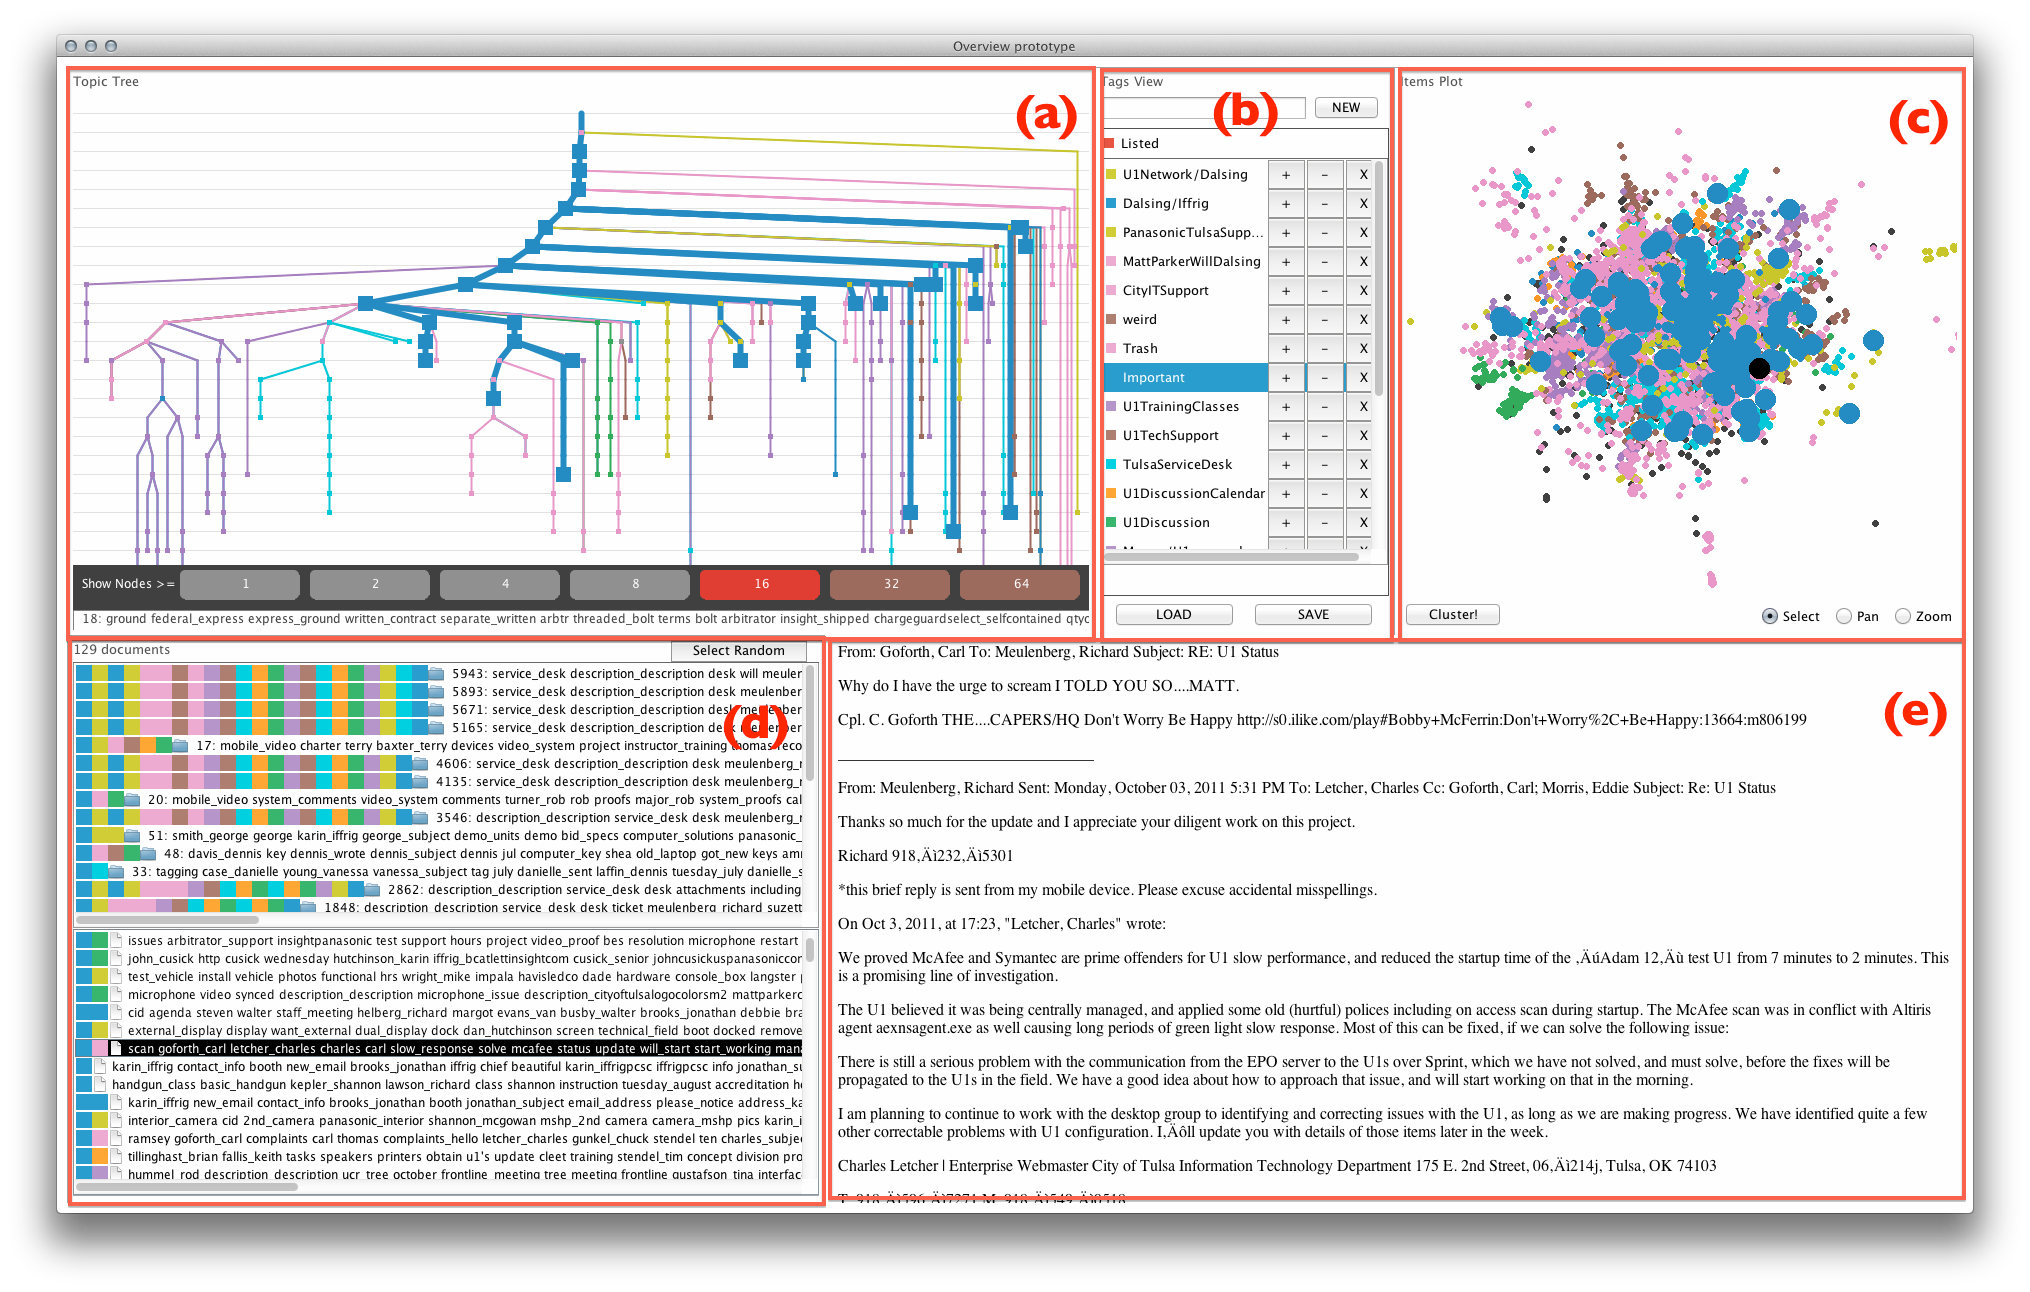
\includegraphics[width=\textwidth]{figures/overview_jw.png}
    \caption
    [
        {\it Overview v2}, displaying {\sc tulsa}'s email corpus.
    ]
    {
        {\it Overview v2}, displaying {\sc tulsa}'s email corpus: (a) a topic tree displays hierarchical clusters of related documents, (b) document tagging functions and a list of user-generated tags, (c) a scatterplot of documents in the corpus; nearby documents are similar, (d) a list of documents having the currently selected tag in (b), (e) an embedded document viewer displaying the currently selected document in (d).
    }
    \label{fig:overview:tulsa}
    \centering
\end{figure}

%-|-|-|-|-|-|-|-|-|-|-|-|-|-|-|-|-|-|-|-|-|-|-|-|-|-|-|-|-|-|-|-|-|-|-|-|-

These were the motivating questions of Jonathan Stray, our collaborator at the Associated Press, who recently worked with our group to develop {\it Overview}\index{Overview (document mining tool)}, a visualization tool to support the process of mining large document corpuses~\cite{Ingram2012}\index{document data}. 
A prototype of {\it Overview}\index{Overview (document mining tool)} was released publicly in early 2012\footnote{\url{https://overviewdocs.com/}}. 
{\it Overview}\index{Overview (document mining tool)}'s user interface, shown in Figure~\ref{fig:overview:tulsa}, is comprised of set of linked views for exploring hierarchical clusters\index{hierarchical data} of related documents\index{document data} within a corpus, providing means for reading documents, as well as for tagging them with personally meaningful terms or phrases. 

Stray believes that the need to mine large document corpuses\index{document data} will increase in the coming months and years, and that current practices made this process impractical. 
These practices gravitated to either keyword searches or brute-force approaches: reading or skimming all documents in a corpus\index{document data}. 
The former approach requires one to know a priori what one is looking for, while the latter is too time-consuming, difficult to streamline and manage. 
In both cases, exploratory analysis is poorly afforded: it is impossible to sample representative documents\index{document data} in a corpus and extract the trends or patterns. 
{\it Overview}\index{Overview (document mining tool)} has been designed to make this exploration possible.

A post-deployment evaluation\index{evaluation} of {\it Overview}\index{Overview (document mining tool)} was an attractive opportunity for both Stray and our research group. 
The project was also well-situated within my larger research goals relating to evaluation\index{evaluation} methodologies and the characterization of exploratory data analysis. 

In the sections that follow, I describe the methodology of my evaluation\index{evaluation}, followed by my current findings. 
Working with a collaborator from outside of academia has been a novel experience; in the final section of this report, I reflect upon the advantages, constraints, and implications of the {\it collaborator-as-gatekeeper} relationship. 
I then look back upon my research process thus far, discussing perceived inefficiencies as well as ideas for future improvement. 
I conclude with thoughts on how this project fits into the larger scheme of my PhD research.
I do not yet claim a defined research contribution, as this paper is intended to be a largely reflective account of an ongoing project.

%-------------------------------------------------------------------------
\subsection{Methodology}
\label{app:overview:prelim-methodology}
%-------------------------------------------------------------------------

My intent of conducting a post-deployment evaluation\index{evaluation} of {\it Overview}\index{Overview (document mining tool)} has been to assess whether or not it meets the exploratory data analysis needs of individuals with large document corpuses\index{document data} and hunches about potential stories contained within them; could {\it Overview}\index{Overview (document mining tool)} make writing a story possible in situations where doing so was previously impossible, or at least highly impractical? 
An evaluation\index{evaluation} would also serve Stray's need to identify major usability issues and barriers to adoption\index{adoption}. 
Finally, given that {\it Overview}\index{Overview (document mining tool)} displays a document corpus\index{document data} using a novel visual encoding\index{visual encoding} design choice~\cite{Ingram2012}, our evaluation\index{evaluation} would also seek to determine if journalists have a conceptual understanding of how this visual encoding\index{visual encoding} represents the structure of semantic relationships in a document corpus\index{document data}.

An ideal research methodology for this work would include in-situ interview and observation sessions, in the spirit of longitudinal insight-based evaluations~\cite{Saraiya2006}\index{evaluation!insight-based evaluation}\index{insight} and multi-dimensional long-term case studies~\cite{Shneiderman2006}\index{case study}.
However, our user base is distributed around the world, and logistical constraints keep me from visiting each individual journalist\index{journalism} in their newsrooms.
Furthermore, like many busy professionals, journalists\index{journalism} are often working under tight deadlines, and have little time to participate in multi-session longitudinal studies. 
As a result, observing and interviewing these journalists\index{journalism} in-situ is infeasible. 
These constraints limit possible data collection methods, which in turn has dictated my choice of methodology, a less than ideal situation. 
Relying upon retrospective accounts of journalists'\index{journalism} experiences with {\it Overview}\index{Overview (document mining tool)}, via in-depth interviews and elicited textual accounts, necessitates an interpretive perspective, a focus on the language journalists\index{journalism} use to describe their processes. 

A grounded theory methodology~\cite{Charmaz2006}\index{grounded theory} appeared to be appropriate, given a need to construct a post-hoc interpretation of journalists'\index{journalism} processes of exploratory data analysis. 
The constant comparative philosophy of grounded theory\index{grounded theory} prompts me to think flexibly, to make comparisons between the process of using {\it Overview}\index{Overview (document mining tool)} with other journalistic processes, with processes relating to exploratory data analysis as it occurs in other domains. 
Comparisons are also made between journalists\index{journalism} and over periods of time, before and after the introduction of {\it Overview}\index{Overview (document mining tool)} into one's workflow\index{workflows}. 
I initially proposed this methodology in an earlier research proposal, which was submitted as a final project for a course in interpretive and critical research, taken in the winter term of 2011/2012. 
This proposal is included in the supplemental material.

I am not the first to adopt a grounded theory\index{grounded theory} methodology and its methods in visualization research. 
The methodology has informed prior work characterizing the use of visualization tools and techniques by professionals in domains such as architecture~\cite{Tory2008} and intelligence analysis~\cite{Kang2011}, as well as our study of processes of high-dimensional data\index{high-dimensional data} analysis \ac{DR}\index{dimensionality reduction (DR)} across multiple domains\footnote{Documented in \autoref{ch:drvistasks}}. 
In evaluation\index{evaluation} research, a ``grounded evaluation'' methodology\index{evaluation} has been used for the in-situ study of a visualization tool's efficacy in a target context of use~\cite{Isenberg2008}.

A further justification for the use of a grounded theory\index{grounded theory} methodology is that my research questions are not theoretically deduced hypotheses, nor is my objective to explicitly validate or refute prior task\index{task} characterizations of data analysis~\cite{Amar2005,Pirolli2009,Springmeyer1992}. 
Rather, my eventual goal is to construct a mid-level, cross-domain task\index{task} characterization. 
Thus my starting point is not a rigid theoretical framework, but with the personal accounts of {\it Overview}\index{Overview (document mining tool)} users.
Of course, no research exists in a void, uninfluenced by previous work. 
As such, my research questions are informed by assumptions and sensitizing concepts held within the visualization community. 
It is these sensitizing concepts that have allowed me to frame data collection methods, particularly a preliminary set of interview questions. 

These sensitizing concepts include the notion that exploratory data analysis occurs in stages~\cite{Pirolli2009}. 
Exploratory data analysis may involve stages of hypothesis generation, without a well-defined set of questions in mind. 
There are also stages of hypothesis validation, where the goal is to support or refute prior evidence. 
Individuals may or may not engage in both types of stages during the course of a single investigation. 

The products of exploratory data analysis are also among my sensitizing concepts. 
These products include moments of {\it insight}~\cite{Chang2009,North2006,Yi2008}\index{insight}, serendipitous discoveries~\cite{Andre2009}, and both optimal and suboptimal solutions to closed- and open-ended problems~\cite{Mayr2010}. 
Admittedly, these products are ill-defined constructs within the language of our research community, and it is necessary for me to attain our participantsÕ interpretations of their meanings, as well as their own terminology.

Finally, these sensitizing concepts include the disentanglement of a data analyst's learned expertise~\cite{Chang2010}. 
By this I mean that an analyst may have expertise related to their domain, expertise using specific analytical tools or techniques, and expertise regarding the data under examination, its semantics, and its provenance.

\bstart{Participant recruitment}
The recruitment of research participants has been difficult to predict, and dependent on the number of individuals who download, install, and use {\it Overview}\index{Overview (document mining tool)} for the purpose of writing a story. 
As a representative of a reputable news agency and a recipient of a prestigious Knight Foundation grant, Stray's clout meant that {\it Overview}\index{Overview (document mining tool)} would be highly visible to the journalism\index{journalism} community. 
Participant recruitment is therefore a matter of waiting for prospective {\it Overview}\index{Overview (document mining tool)} users to establish contact with Stray. 
This means that he acts as a gatekeeper to research participants, an aspect of this project that I reflect upon later in the discussion section.

\bstart{Data collection}
My primary data collection method is that of an in-depth, open-ended interview, recorded for later transcription. 
Following the methodology of grounded theory~\cite{Charmaz2006}\index{grounded theory}, I have not specified the number of interviews that I planned to conduct a priori. 
The final number of interviews will depend upon how many {\it Overview}\index{Overview (document mining tool)} users express a willingness to participate in interviews and upon whether and when data saturation occurs, which I discuss in the following section. 

Multiple interviews with each participant would be ideal, as processes change over the course of an investigation. 
However, this is an unrealistic plan; as mentioned above, journalists\index{journalism} often conduct their investigation and write articles under tight deadlines, and often only have the spare time required to commit to an intensive interview after their story is written. 

Regarding the content of these interviews, I began with a short list of interview foci and a small set of representative questions for each, composed according to guidelines for open-ended interviews~\cite{Fontana1994} and for interviews conducted in the context of a grounded theory study~\cite{Charmaz2006}\index{grounded theory}. 
These foci correspond with the sensitizing concepts described above. 
I ground the interview in the current document corpus\index{document data} under investigation, inviting comparisons from the interviewee's prior body of work, before using {\it Overview}\index{Overview (document mining tool)}. 
This list of foci and questions, included in this report's supplemental material, is flexible and subject to change, owing to the possibility that early interviews illuminate unanticipated concepts.

I compliment interviews by gathering texts and other information from participants, such as {\it Overview}\index{Overview (document mining tool)}'s log file of timestamped interface interactions\index{interaction!interaction logs}. 
I also gather information regarding their data, such as the format and number of documents\index{document data} contained in the corpus under investigation. 
Finally, I request copies of notes participants take during the course of their investigation.
Journalists'\index{journalism} notes are less intrusive than dedicated progress or insight reports~\cite{Rester2007a,Saraiya2006}\index{evaluation!insight-based evaluation}\index{insight}; they are personalized and externally valid, offering yet a another window into their own interpretations of their investigative process.
 
\bstart{Data analysis}
Data collection and analysis occur concurrently. 
I subject interview transcripts and textual artifacts collected from journalists\index{journalism} to multiple iterations of coding\index{coding (qualitative data analysis)}, wherein I call upon the constant comparative method, the basis of grounded theory\index{grounded theory}. 
First, {\it initial coding}\index{coding (qualitative data analysis)} labels excerpts from transcripts and notes with words from the participant's own vocabulary, using an active voice to emphasize a focus on a process occurring in time~\cite{Charmaz2006}. 
Next, I generate tentative categories of codes, each with an explanatory rationale based on comparisons between code instances, recorded as memos. 
This process informs subsequent data collection and the process of {\it focused coding}\index{coding (qualitative data analysis)}, wherein I re-code the data using emerging categories. 

%-|-|-|-|-|-|-|-|-|-|-|-|-|-|-|-|-|-|-|-|-|-|-|-|-|-|-|-|-|-|-|-|-|-|-|-|-

\begin{figure}
    \centering
    \fbox{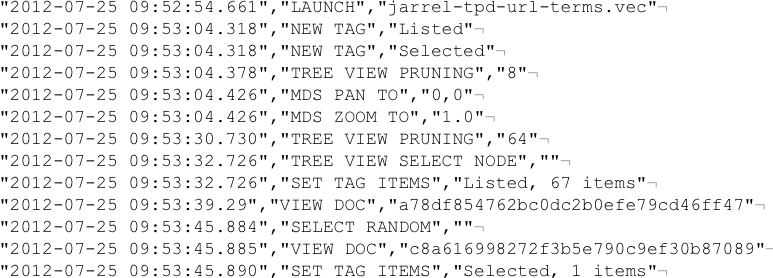
\includegraphics[width=0.975\textwidth]{figures/overview_log.png}}
    \caption
    [
        An excerpt of {\it Overview}'s log file, listing timestamped interaction events.
    ]
    {
        An excerpt of {\it Overview}'s log file, listing timestamped interaction events, such as tagging a document or tree node, panning or zooming within the scatterplot, or viewing documents.
    }
    \label{fig:overview_log}
    \centering
\end{figure}

%-|-|-|-|-|-|-|-|-|-|-|-|-|-|-|-|-|-|-|-|-|-|-|-|-|-|-|-|-|-|-|-|-|-|-|-|-

As categories are refined and theoretical concepts emerge through the process of focused coding\index{coding (qualitative data analysis)}, I may reach a point of theoretical saturation, when no major unexamined concepts are expected to appear as a result of future data collection. 
At this time, a mid-level task\index{task} characterization of exploratory data analysis in this domain may begin to emerge. 
This stage will also invite comparisons between my nascent theory and existing theories~\cite{Amar2005,Pirolli2009,Springmeyer1992}.

Extensive log file analysis is complimentary to the analysis of transcripts and textual artifacts, providing me with a partial yet objective account of usage strategy~\cite{Pohl2010}. 
After parsing, aggregating, and filtering events in the log, I can extract descriptive usage statistics. 
The log file, as shown in Figure~\ref{fig:overview_log}, 
reveals how many documents were viewed and tagged during the course of a user's investigation, as well as how various user interface features were used over time.

%-------------------------------------------------------------------------
\subsection{Findings}
\label{app:overview:prelim-findings}
%-------------------------------------------------------------------------

To date, two professional journalists\index{journalism} and a pair of academic researchers have completed an analysis of a large document corpus\index{document data} using {\it Overview}\index{Overview (document mining tool)}. 
I am also aware of several additional journalists\index{journalism} and academic researchers who may be currently using it. 
Finally, I am aware of a journalist\index{journalism}, an academic researcher, and business consultant who abandoned use of {\it Overview}\index{Overview (document mining tool)}, as it either did not meet their needs or was incompatible with their existing workflow\index{workflows} or set of tools.

The discovery of prospective users from fields outside of journalism\index{journalism} was unanticipated, indicating that {\it Overview}\index{Overview (document mining tool)} may support exploratory data analysis in the digital humanities\index{digital humanities}, communications\index{communications}, and related domains.

\bstart{Case study}
Of the two journalists\index{journalism} who completed an analysis of a document corpus\index{document data} using {\it Overview}\index{Overview (document mining tool)}, one published his findings~\cite{Wade2012}. The {\sc tulsa} journalist\index{journalism} was willing to be interviewed, and he provided us with not only his log file, but also his entire dataset. 
He also kept thorough notes during his investigation, and would later write a blog post intended for prospective {\it Overview}\index{Overview (document mining tool)} users~\cite{Wade2012a}. 
In many ways, he was an ideal research participant, and I should not expect the same amount and depth of information from all future participants. 

Beginning with an anonymous tip and hunch relating to a botched, four million dollar police equipment purchase, the {\sc tulsa} journalist\index{journalism} accumulated a document corpus\index{document data} of 5,996 Tulsa Police Department emails via a municipal records request. 
Using {\it Overview}\index{Overview (document mining tool)}, the journalist\index{journalism} discovered newsworthy evidence contained in only a handful of emails: several police officials were responsible for the poorly managed purchase, and were caught in a potential conflict of interest with an equipment supplier.

I interviewed the {\sc tulsa} journalist\index{journalism} three days after his story ran. 
The two-hour interview was conducted via a Google$^+$ Hangout video chat, a service that also affords chat participants the ability to share their screen. 
This feature permitted the {\sc tulsa} journalist\index{journalism} to walk us through his process, both with and without {\it Overview}\index{Overview (document mining tool)}. 
Using a screen capture application, I recorded the {\sc tulsa} journalist's video feed along with the audio conversation. 
I later transcribed this interview, whereupon I realized that the ratio of time spent transcribing to interview duration was approximately four to one. 
I then coded this transcript, alongside the {\sc tulsa} journalist's\index{journalism} notes, according to the initial coding\index{coding (qualitative data analysis)} scheme described above.
Meanwhile, my analysis of the {\sc tulsa} journalist's\index{journalism} log file provided an objective account of his process, corroborating with his subjective, retrospective description.
With over twenty thousand events logged, log analysis was exhaustive yet time-consuming, requiring the better part of a week to complete; 
I reflect upon the utility and duration of log analysis in the following section.

The {\sc tulsa} journalist\index{journalism} has only been on the Tulsa ``cops beat'' for a couple of years. 
While he considers himself to be tech-savvy, he has no formal background in programming or visualization. 
As such, he required a considerable amount of assistance while installing and configuring {\it Overview}\index{Overview (document mining tool)}. 
This story was, in his words, the biggest story of his early career. 
The only similar story in his prior body of work was one about the emergency response practices of a local college security force, an investigation that necessitated the examining of a two-foot high stack of emergency call log printouts, while making annotations with highlighters. 

What was most fascinating about the {\sc tulsa} journalist's\index{journalism} process was his determination to read and tag most of the documents\index{document data} in the corpus. 
In 56 hours of use, spread over 15 non-consecutive days, an impressive 70\% of the documents\index{document data} in the corpus were selected and viewed in {\it Overview}\index{Overview (document mining tool)}'s embedded document viewer for at least one second. 
Rather than use {\it Overview}\index{Overview (document mining tool)} as a means of broadly exploring and sampling documents\index{document data} within a corpus, the {\sc tulsa} journalist's\index{journalism} usage strategy defied expectation:

\begin{quote} 
    {\it ``At the worst I wanted to use (Overview) as a way of organizing me looking through every email, and at best I wanted to look at most of the emails.''}
\end{quote}

A systematic and efficient process was a recurring theme in the interview: the quick dismissal of uninteresting or irrelevant documents, the worry about overlooking important documents, the prevention of having to re-read documents, and the vigilant scanning for unique or ``rogue'' documents. 
Always conscious of deadlines quotas, the {\sc tulsa} journalist\index{journalism} wanted to streamline his process of viewing documents as much as possible, at times referring to his rate of skimming individual documents as a ``speed test'':

\begin{quote}
    {\it ``The speed factor, you're talking about just clicking and glancing, it could literally be as fast as three seconds per email. Until I got to one that I needed to know...''}
\end{quote}  

Figure~\ref{fig:overview_jw_results} shows that during the first several sessions of the {\sc tulsa} journalist's\index{journalism} investigation.
Longer median document viewing times reflects the process of getting an initial feel for the documents contained in the corpus\index{document data}.
During the longer sessions that followed, shorter median document viewing times reflected his streamlined, exhaustive scouring of the corpus. 
While finalizing his investigation, fewer documents were read for longer periods of time; returning to a smaller number of significant documents. 
By this time he was preparing to write his article.  

%-|-|-|-|-|-|-|-|-|-|-|-|-|-|-|-|-|-|-|-|-|-|-|-|-|-|-|-|-|-|-|-|-|-|-|-|-

\begin{figure}
    \centering
    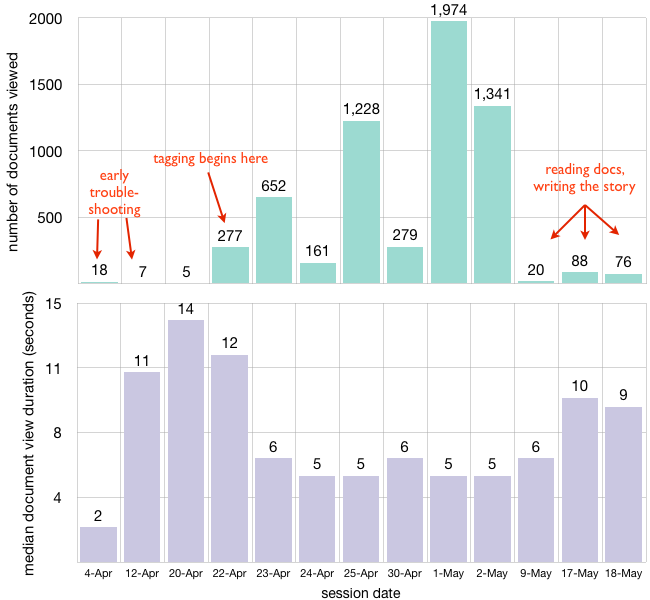
\includegraphics[width=\textwidth]{figures/overview_jw_results.png}
    \caption
    [
        The median time spent viewing a single document.
    ]
    {
        The median time spent viewing a single document was lower during sessions in which more documents were viewed.
    }
    \label{fig:overview_jw_results}
    \centering
\end{figure}

%-|-|-|-|-|-|-|-|-|-|-|-|-|-|-|-|-|-|-|-|-|-|-|-|-|-|-|-|-|-|-|-|-|-|-|-|-

The {\sc tulsa} journalist's\index{journalism} similarly completist use of {\it Overview}\index{Overview (document mining tool)}'s document tagging feature may have implications for information management in exploratory data analysis tools. 
He created twenty-two tags, tagging 92\% of the documents in the corpus\index{document data} with at least one of them. 
He explained that he became ``obsessed'' with having every document tagged. 
This came at the expense of having a complicated, cross-cutting, and disorganized set of tags. 
Regarding his tags, it was clear that eighteen of them reflected the content of the documents\index{document data}: email subject, sender, or recipient. 
The remaining four tags reflected a document's level of importance ({\it Important, Trash}) or personal memo for follow-up ({\it Check on} [this]{\it, Weird}). 
He explained that he would have additionally liked to have had {\it unread / read} and {\it relevant / not relevant} flags for each document. 
The latter four tags and flags cross-cut the eighteen content-based tags, and suggest that two strategies of information management were being used during his investigation. 

All things considered, could the {\sc tulsa} journalist\index{journalism} have carried out his investigation without {\it Overview}\index{Overview (document mining tool)}? 
He admitted the possibility, however it would have taken an estimated four months of full-time dedication to read the entire corpus, while maintaining the same level of organization that {\it Overview}\index{Overview (document mining tool)} provided him. 
By contrast, his investigation using {\it Overview}\index{Overview (document mining tool)} took less than two weeks. 
With news agency deadlines and article quotas to consider, a longer-term project would have been relegated to a part-time assignment; upon its completion, the story would have run the risk of no longer being newsworthy.

%-------------------------------------------------------------------------
\subsection{Discussion}
\label{app:overview:prelim-discussion}
%-------------------------------------------------------------------------

The post-deployment study of {\it Overview}\index{Overview (document mining tool)} is far from over. 
At present, I have only spoken in depth with a single user, one who may not be representative of all {\it Overview}\index{Overview (document mining tool)} users. 
Finding users with different goals and strategies will take time, patience, and a reliance upon Stray as a collaborator. 
In the meantime, I can reflect upon what I've learned and refine my processes of data collection and analysis.

\bstart{Samplers and completists} 
{\it Overview}\index{Overview (document mining tool)} was built for the purpose of broad exploration, sampling documents in a corpus as a means to extract trends or irregularities.
It came as a surprise to both Stray and myself that {\it Overview}\index{Overview (document mining tool)} would instead be used for performing an exhaustive and systematic search.
The {\sc tulsa} journalist's\index{journalism} search criteria was approximate, as opposed to exact, necessitating exploration rather than processes such as keyword search, browsing, or navigating.
Broad sampling and exhaustive approximate search are two usage strategies, both being variants of exploratory data analysis.

I presented a comprehensive analysis of the {\sc tulsa} journalist's\index{journalism} use of {\it Overview}\index{Overview (document mining tool)} to Stray, whereupon we conjectured that the {\sc tulsa} journalist's\index{journalism} usage strategy reflected his initial records request, which was filtered a priori to emails with specific senders, recipients, and subject lines. 
His task\index{task} was to find the small number of ``smoking gun'' emails, those containing the evidence needed for his story, validating the hypotheses that emanated from the original anonymous tip. 

A sample-based usage strategy might arise in cases where the document corpus\index{document data} is ``leaked'' or ``dumped'', rather than requested. 
In the case of document leaks such as the Iraqi war logs~\cite{Stray2012}\footnote{This is a reference to the {\sc iraq-sec} case study\index{case study}; see \autoref{overview:case-studies}.}, a journalist\index{journalism} may explore the corpus broadly, reading far less than 70\% of the corpus in an attempt to attain a gist or summary of its contents, rather than seek the ``smoking gun''. 
Instead, the {\sc tulsa} journalist\index{journalism} was a completist, one who used {\it Overview}\index{Overview (document mining tool)} as a tool for performing an exhaustive, ``I have to read everything'' investigation, albeit more systematically and efficiently than that of his earlier story involving the two-foot stack of call log printouts. 
It also remains to be seen if strategies of information management via tagging used during an exhaustive investigation are also called upon by those using {\it Overview}\index{Overview (document mining tool)} for a more sampling-based analysis of a document corpus\index{document data}.

At this point, I would like to interview an individual who uses {\it Overview}\index{Overview (document mining tool)} with a sample-based strategy, preferably one working with an unfiltered document corpus\index{document data} emanating from a dump or leak. 
Should they have an intention to determine the major trends or themes within, I would be curious to compare their process against that of the {\sc tulsa} journalist's\index{journalism}. 

\bstart{The collaborator as gatekeeper}
Collaborating on a project with non-academic visualization tool builders has well-known advantages and disadvantages~\cite{Sedlmair2011}. 
In my case, a robust, publicly-available tool was completed and deployed before the evaluation\index{evaluation} project began. 
As mentioned above, Stray's professional visibility would also attract potential adopters within the journalism\index{journalism} community. 
As a junior visualization researcher, I do not have sufficient clout within the journalism\index{journalism}, digital humanities\index{digital humanities}, or related communities to attract users. 
It is furthermore inappropriate to evaluate\index{evaluation} the utility of {\it Overview}\index{Overview (document mining tool)} with undergraduate student volunteers or those not working in domains that do not regularly encounter large document corpuses\index{document data}. 
As a result, our collaborator is the gatekeeper to prospective research participants.

But is reputation enough to attract users? In the six months since {\it Overview}\index{Overview (document mining tool)}'s launch, we are aware of only a handful of individuals that have used it, with only one journalist\index{journalism} using it to write a story. 
The time commitment of mining large document corpuses\index{document data} is extensive, not including the time required to install, configure, and learn how to use a new tool such as {\it Overview}\index{Overview (document mining tool)}. 
These problems may be alleviated in a forthcoming release of the {\it Overview}\index{Overview (document mining tool)} web application, which will feature a simplified user interface and a reduced feature set. 
It will also eliminate the need for a desktop installation, requiring less initial configuration. 
I hope that this upcoming release will attract a larger pool of prospective users, providing me with  needed research participants.

\bstart{Reflections on research process}
After many hours spent analyzing the {\sc tulsa} journalist's\index{journalism} interview transcript and log file, I asked myself: what is the value of my analysis efforts? 
Is the log file a trove of information or a rathole? 
I admit that I became distracted by the notion that my findings would have an impact on {\it Overview}\index{Overview (document mining tool)}'s future design. 
It was around this time that Stray revealed plans to remove major features and overhaul the user interface in the forthcoming release of the {\it Overview}\index{Overview (document mining tool)} web application; I believed that my in-depth analysis could validate or refute these design decisions. 
I lost focus on the larger goal of understanding how {\it Overview}\index{Overview (document mining tool)} was used in the process of exploratory data analysis. 
This larger understanding of a process is not interface-specific~\cite{Beaudouin-Lafon2004}; when we understand the process and its interactions, we can then evaluate\index{evaluation} specific interface components.

Ultimately, Stray was fascinated by the detail and depth of my findings, but agreed that it was overkill for the purposes of validating design decisions or for identifying usability issues. 
What mattered most to him was that {\it Overview}\index{Overview (document mining tool)} had been used to write a story, and unexpectedly, that it had been used as a tool for streamlining an exhaustive search, rather than for its intended purpose, being a broad, sample-based variant of exploratory data analysis.

I have been rethinking my data collection and analysis methods, my methodology, and how my findings will eventually be presented to the research community. 
At the level of data collection, I have refined my interview foci to include a deeper examination of the difference between exploratory sampling and approximate search. 
More questions relating to information management and tag usage will also be added. 
At the level of methodology, the major question is whether to continue with a grounded theory\index{grounded theory} approach and its constant comparative, bottom-up philosophy, or to instead survey a broad range of {\it Overview}\index{Overview (document mining tool)} users and then select specific case studies\index{case study} that appear to be radically different, given the users' goals. 
I could imagine reporting on cases of differing usage strategy (broad sampling vs. exhaustive approximate search), corpus provenance (records request vs. leak / dump), or user domain (journalism\index{journalism} vs. digital humanities\index{digital humanities} research). 
When presenting my findings, whichever approach taken will need to be consistent and well-justified.

\bstart{This project in context}
A replicable evaluation\index{evaluation} of a visualization tool that supports the process of exploratory data analysis requires a methodology grounded in a abstract characterization of what this process is and what it is not, an understanding of the form that this process takes across multiple domains. 
My current project is a small part of this dependency, in that it allowed me to study the use of visualization tools or techniques in a single domain.
Over time, I will study exploratory data analysis and the use of visualization tools or techniques in other domains, both personally and via my ongoing comprehensive review of the literature.

I have already adopted multiple data collection and analysis methods; others will surely follow, subject to practical constraints and assessments of expected utility.
A useful evaluation\index{evaluation} methodology and a mid-level task\index{task} characterization are mutually dependent, and will develop together with further study.

%-------------------------------------------------------------------------
\subsection{Conclusion and Future Work}
\label{app:overview:prelim-conclusion}
%-------------------------------------------------------------------------

I am currently continuing my study and evaluation\index{evaluation} of {\it Overview}\index{Overview (document mining tool)}, a tool built for exploring large text document corpuses\index{document data}. 
I've still got a long way to go: in my first completed case study\index{case study}, I observed the tool being used for conducting an exhaustive approximate search; not exactly what I was expecting, but an interesting finding nonetheless. 

I expect to interview more {\it Overview}\index{Overview (document mining tool)} users in the coming weeks and months.
There is also likely to be an opportunity to elicit participation from journalism\index{journalism} students as they use {\it Overview}\index{Overview (document mining tool)} in the context of a course project. 
Such an opportunity would be logistically simpler than observing professional journalists\index{journalism}, affording multi-session in-situ interview and observation methods~\cite{Chang2010,Saraiya2005b}.

Along the way I've learned and reflected upon a great deal: methodological considerations, the process and pitfalls of mixed-method data collection and analysis, and my experience working with an external collaborator. 
Writing this report has served to get my thinking directed toward my larger goal: the continued study of visualization evaluation\index{evaluation} and exploratory data analysis.

%-------------------------------------------------------------------------
%-------------------------------------------------------------------------

\section{Overview v3}
\label{app:overview:v3}

%-------------------------------------------------------------------------
%-------------------------------------------------------------------------

\textsl{Overview v3}, a web-based application released in Fall 2012, is shown in \autoref{app:overview:fig:overview-v3}.

%-|-|-|-|-|-|-|-|-|-|-|-|-|-|-|-|-|-|-|-|-|-|-|-|-|-|-|-|-|-|-|-|-|-|-|-|-

\begin{figure}
	\centering
	\fbox{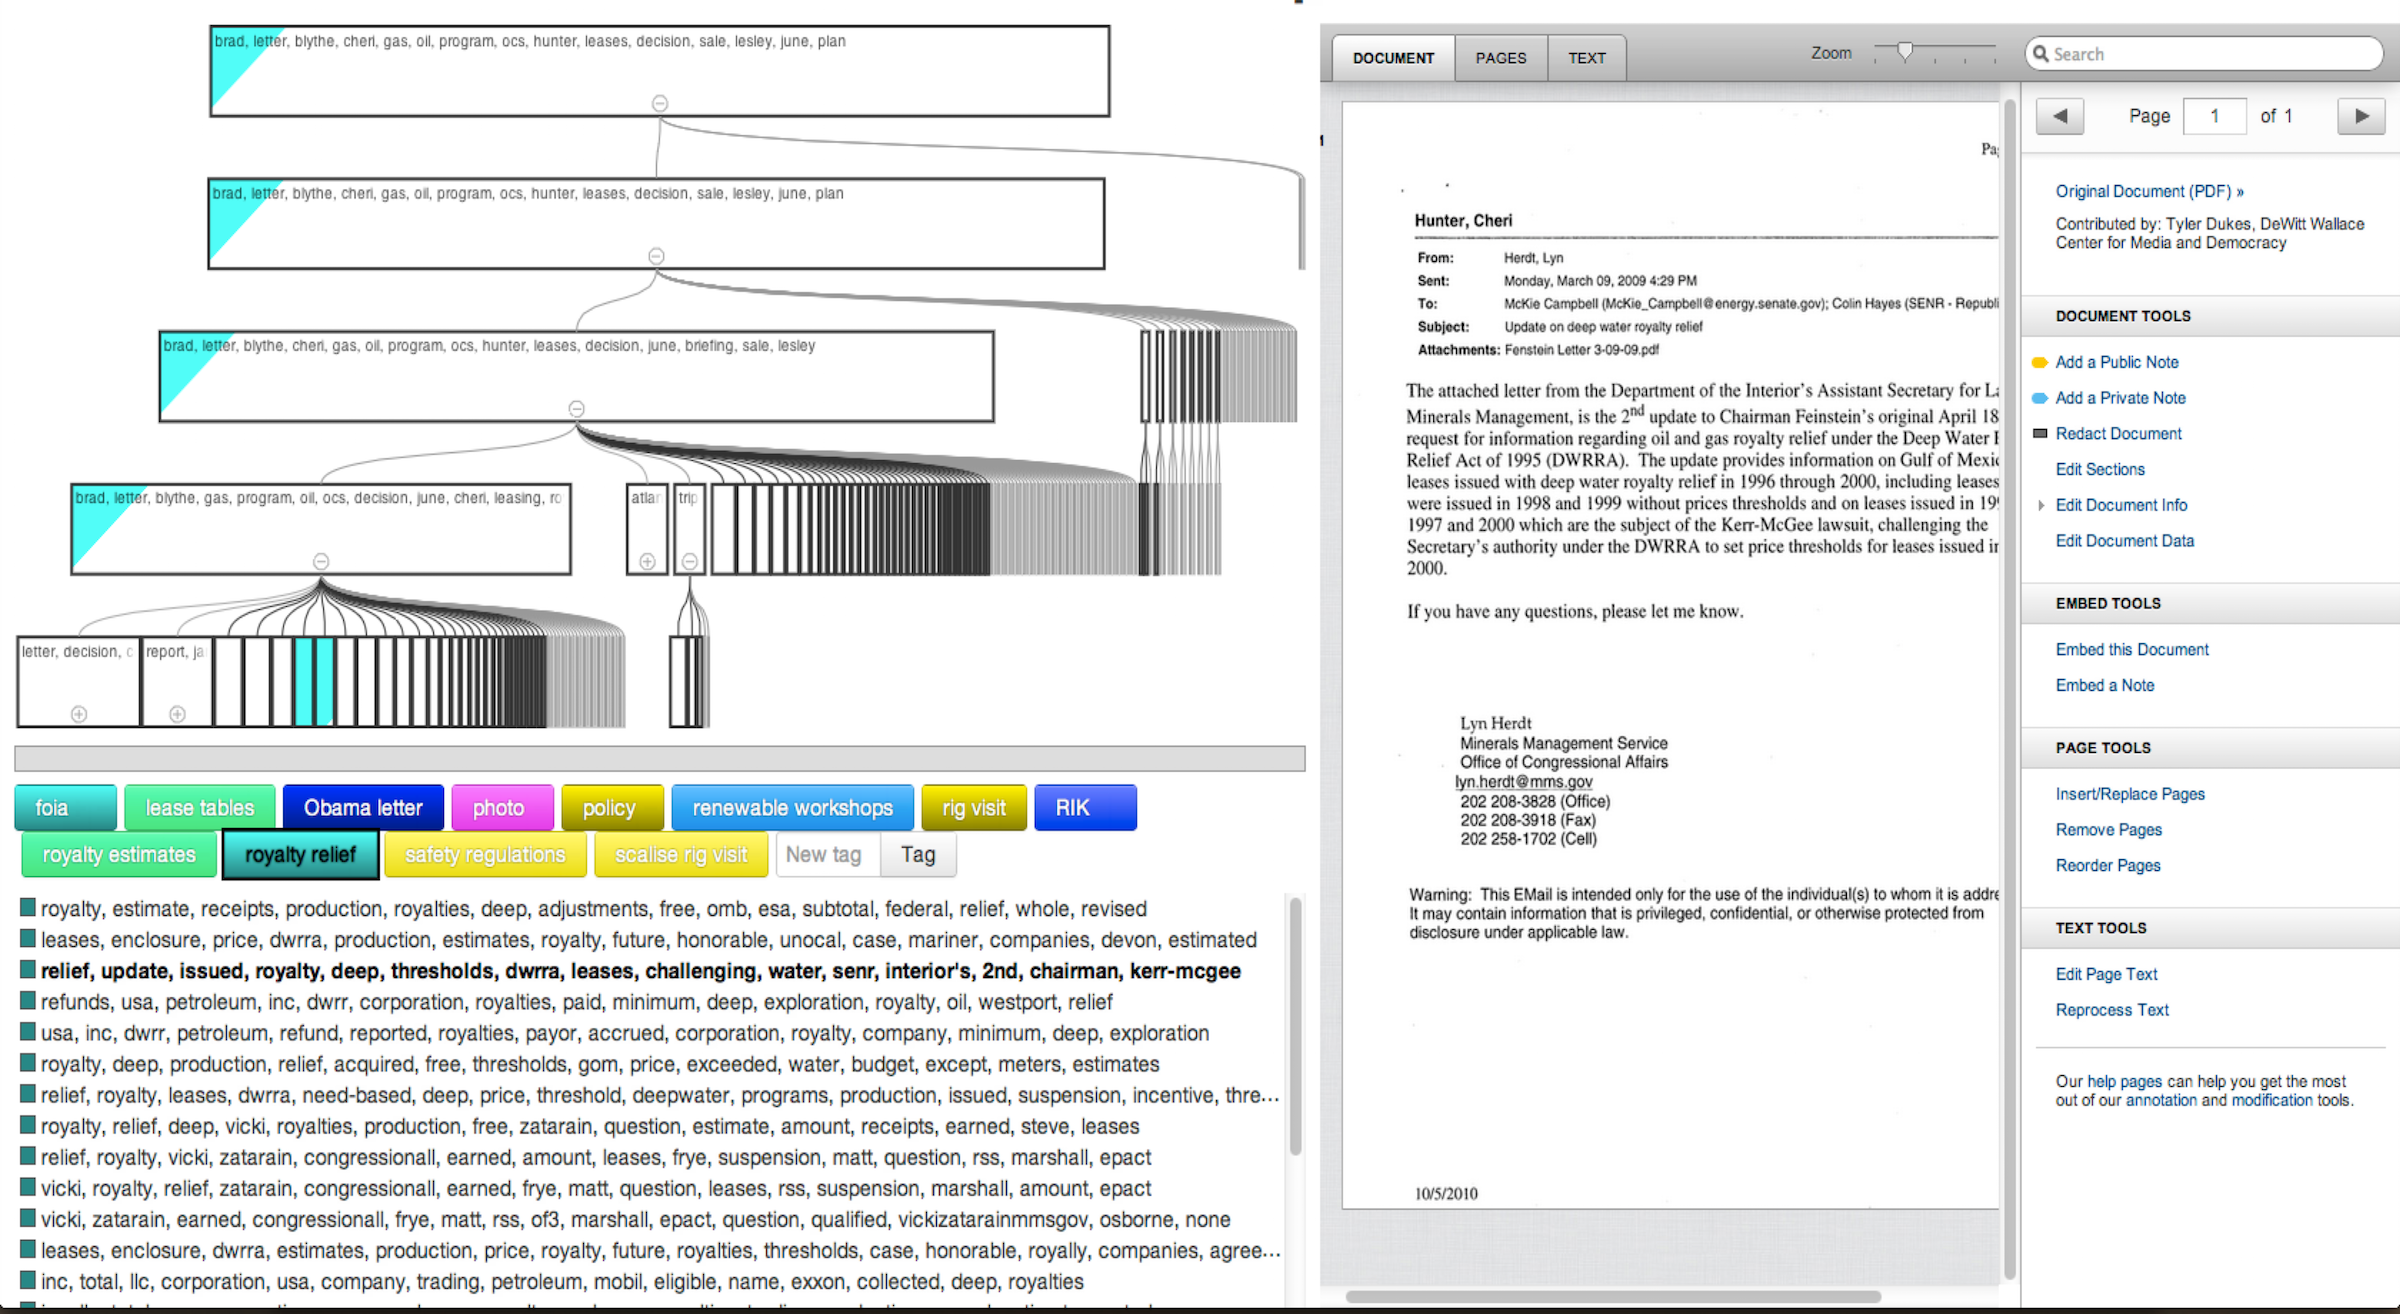
\includegraphics[width=0.975\textwidth]{figures/overview-v3.png}}
	\caption
	[
	    \textsl{Overview v3}, a web-based application released in Fall 2012.
	]
	{
    	\textsl{Overview v3}, a web-based application released in Fall 2012.
	}
	\centering
	\label{app:overview:fig:overview-v3}
\end{figure}

%-|-|-|-|-|-|-|-|-|-|-|-|-|-|-|-|-|-|-|-|-|-|-|-|-|-|-|-|-|-|-|-|-|-|-|-|-